\subsection{Modelling relevant aspects in EA}
\visHeader

The first step is to load an existing metamodel into EA. A complete and automatic import of existing Ecore files in EA is currently not possible and therefore,
\emph{relevant parts} of the existing metamodel (\texttt{GenModel}) have to be modelled manually. Although this might sound frightening (especially for
large, complex metamodels), the emphasis here on \emph{relevant} indicates that only elements that are needed for the transformation have to be present in
EA, where more can be added iteratively as the transformation grows. 

If you find this section challenging or unclear, refer to Part II: Ecore for a detailed review of metamodel construction.

\begin{enumerate}

\item[$\blacktriangleright$] Open Eclipse and create a new metamodel project named \texttt{Ecore\-To\-Gen\-Model}, selecting the \texttt{Add Demo Specification}
option in the project wizard window.

\item[$\blacktriangleright$] A new specifications folder with the project name should have loaded into the workspace, along with an \texttt{DemoTestSuite} JUnit
test. You may choose to either delete or ignore this second project -- it is used as the example in Part I and is irrelevant in this context.

\item[$\blacktriangleright$] Double-click the generated \texttt{Ecore\-To\-Gen\-Model.eap} file to open your project in EA. Explore the project browser and
make of note of the packages already present in EA under \texttt{eMoflon Languages}, especially \texttt{Ecore} which we shall use in this transformation.

\item[$\blacktriangleright$] Select either root note and create a new package named \texttt{Gen\-Model\-Language}. 

\item[$\blacktriangleright$] Add a new Ecore diagram and model the elements as depicted in Fig.~\ref{fig_gMM}. You'll need to create the three EClasses on
the left, but \texttt{Ecore::EPackage} and \texttt{Ecore::EClass} can be drag-and-dropped and pasted as links from the project browser. 

\vspace{0.5cm}

\begin{figure}[htbp]
\begin{center}  
	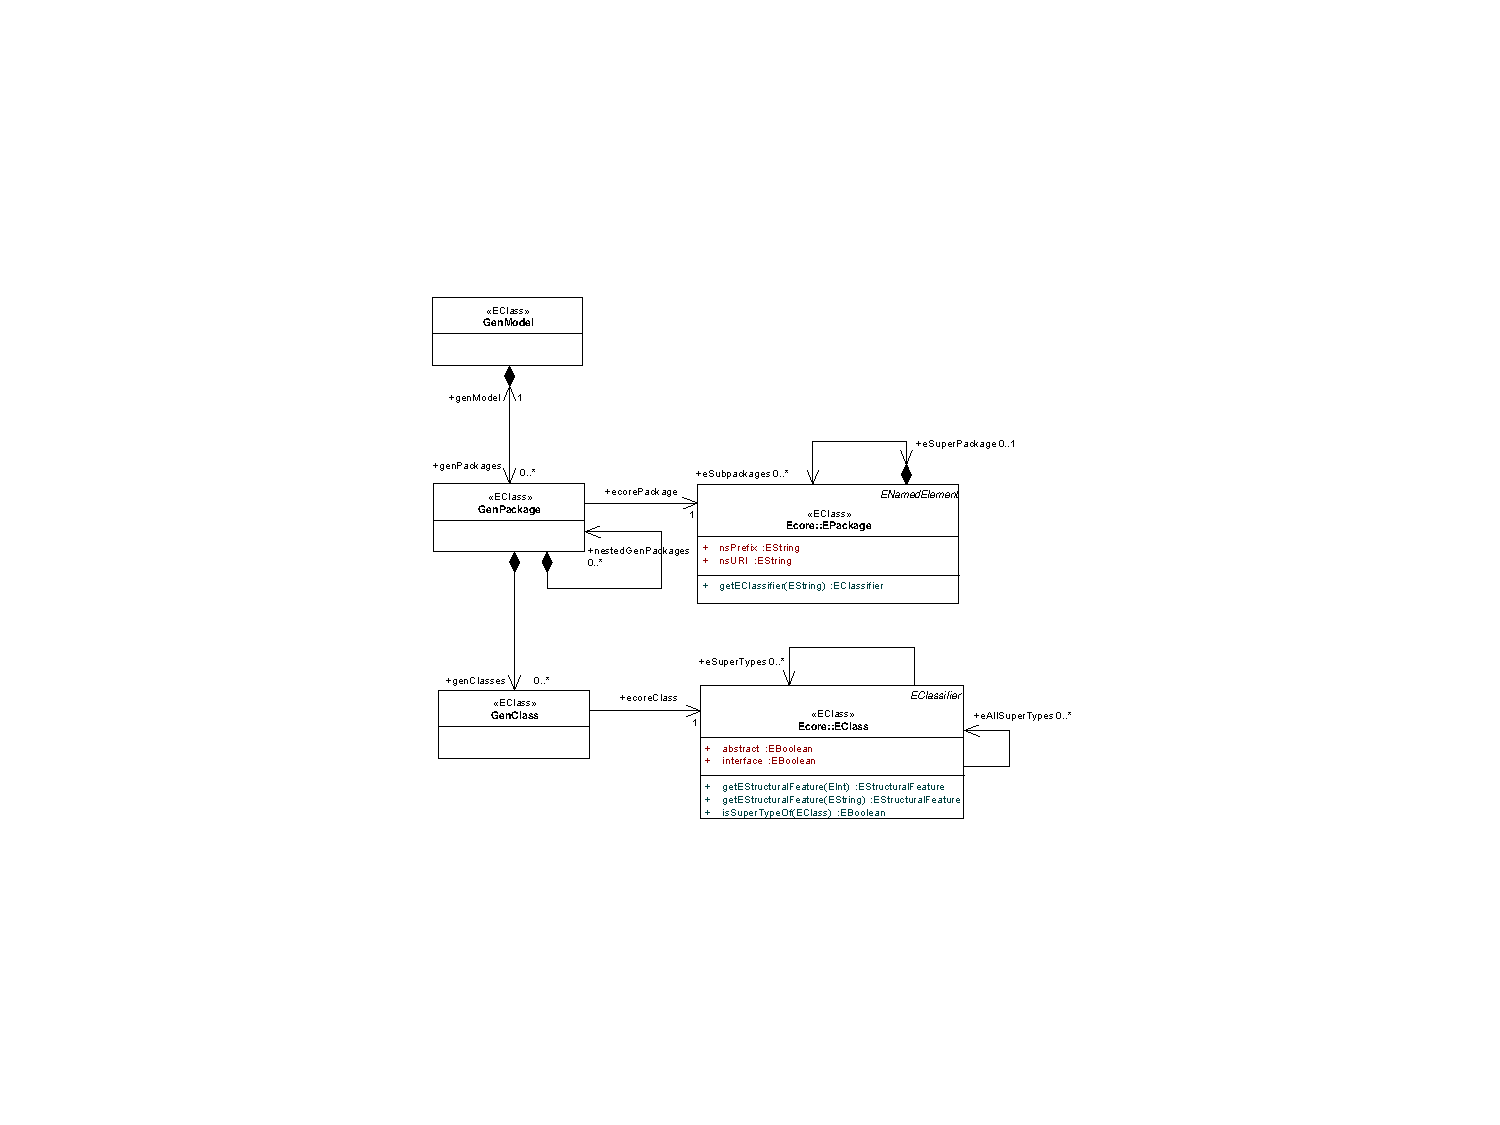
\includegraphics[width=\textwidth]{CDGenmodel.pdf}
	\caption{Metamodel of \texttt{GenModel}}  
\label{fig_gMM}
\end{center}
\end{figure} 

\vspace{0.5cm}

\item[$\blacktriangleright$] Please note that the actual \texttt{GenModel} metamodel contains many more elements, but this subset is sufficient for our
task.

\item[$\blacktriangleright$] Navigate to the project browser again and create another packaged named \texttt{Ecore2GenModel}.  This will contain the
\texttt{Transformer} class; Complete its diagram as depicted in Fig.~\ref{fig_e2gm}.

\item[$\blacktriangleright$] Carefully double-click each method to create and implement their SDMs as depicted in Figs.~\ref{fig_pack2gm} and \ref{fig_transf}.
\end{enumerate}

\newpage

\vspace*{2cm}

\begin{figure}[htbp]
	\begin{center}  
	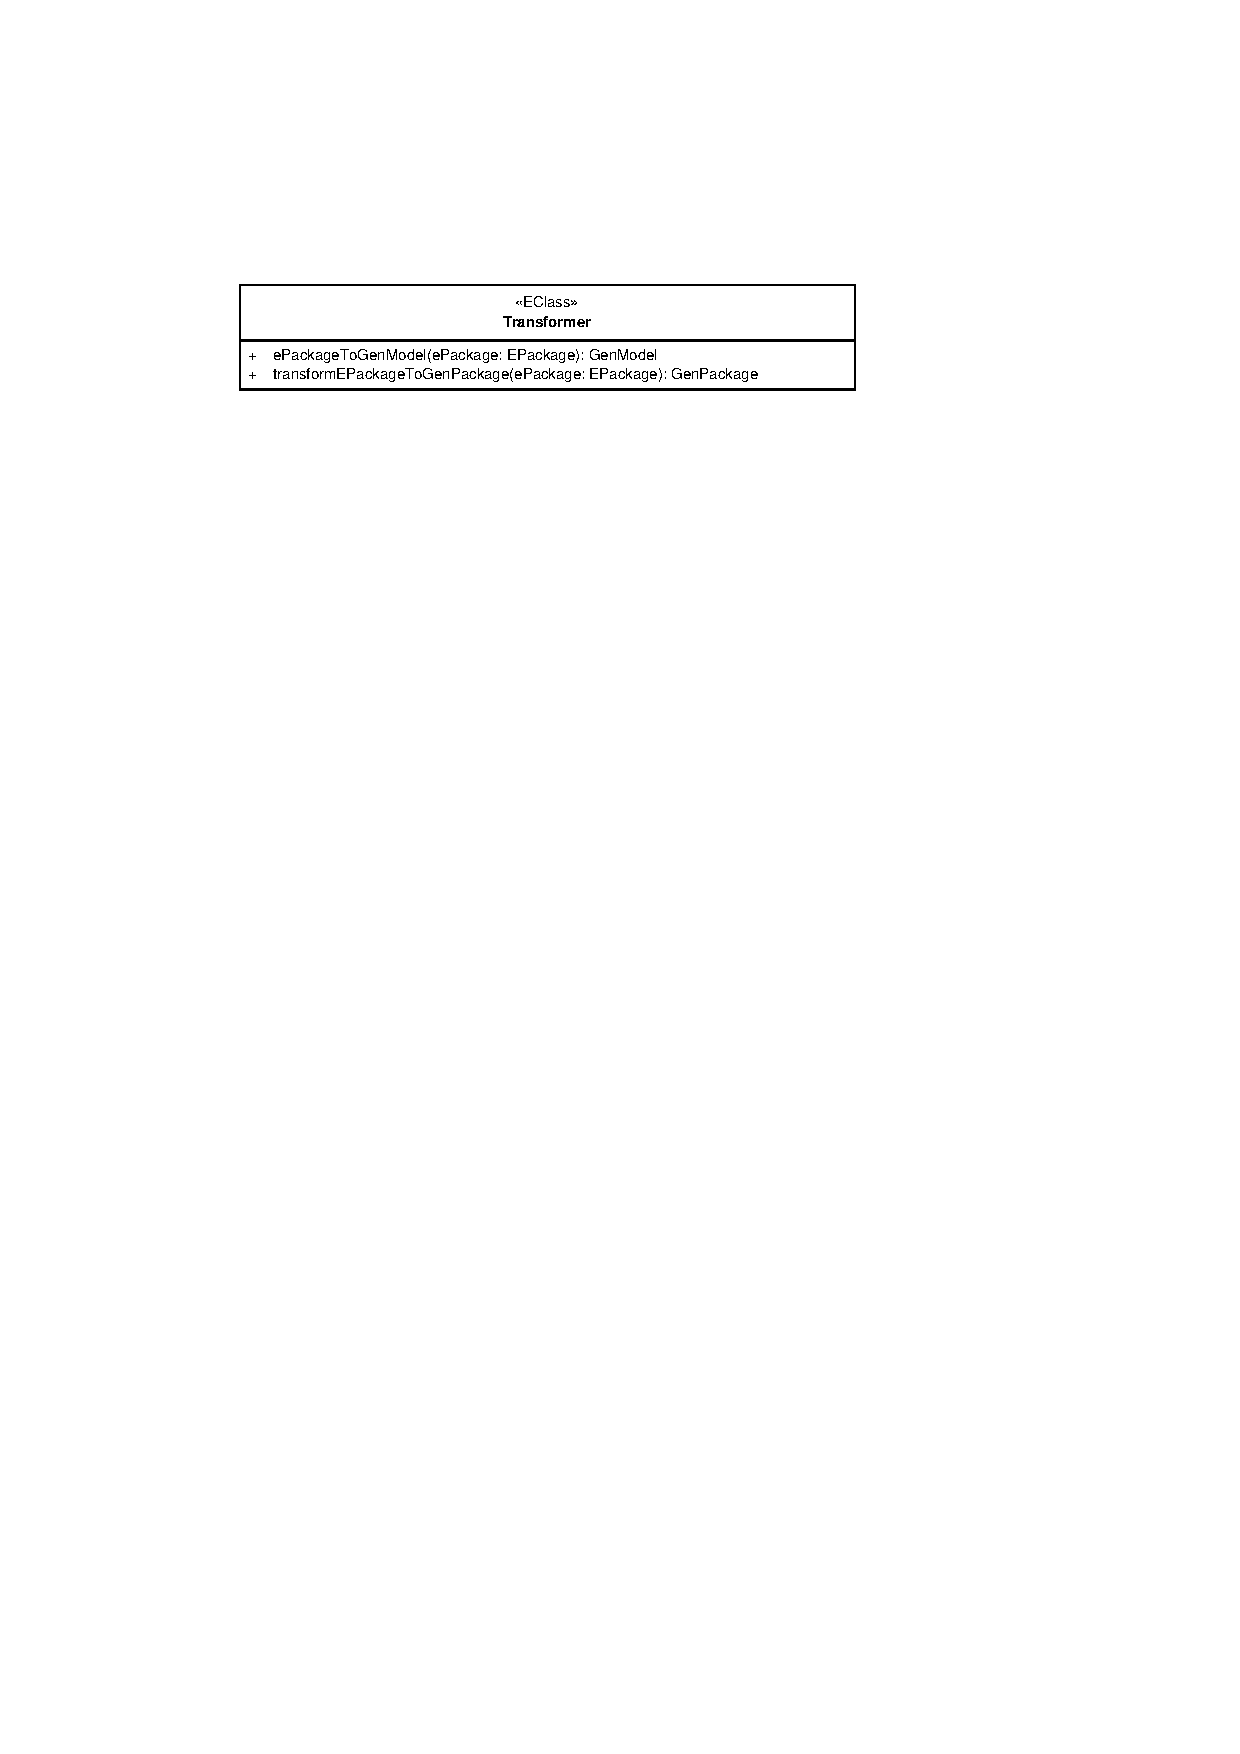
\includegraphics[width=0.7\textwidth]{CDTransformer.pdf}
	\caption{Methods in \texttt{Transformer}}  
	\label{fig_e2gm}
	\end{center}
\end{figure} 

\vspace{1cm}

\begin{figure}[htbp]
\begin{center}  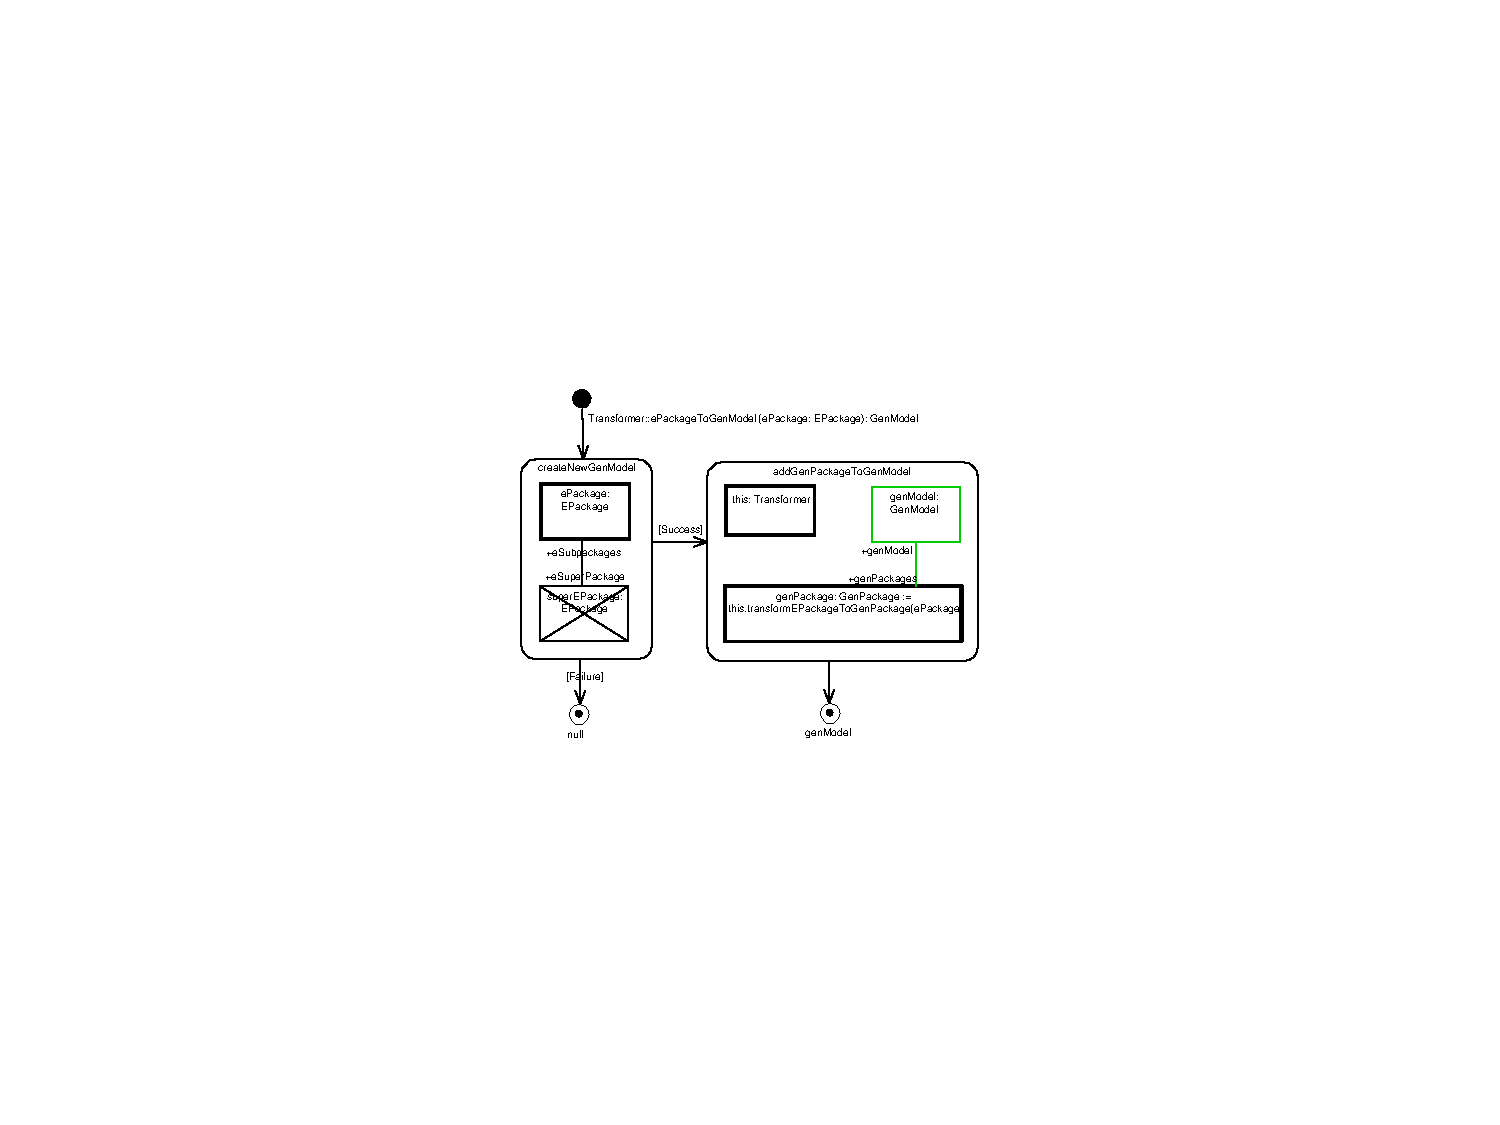
\includegraphics[width=0.8\textwidth]{SDMePackageToGenModel.pdf}
        \caption{Main method for \texttt{EPackage} to \texttt{GenModel} transformation}  
  \label{fig_pack2gm}
\end{center}
\end{figure} 

\begin{figure}[htbp]
\begin{center}  
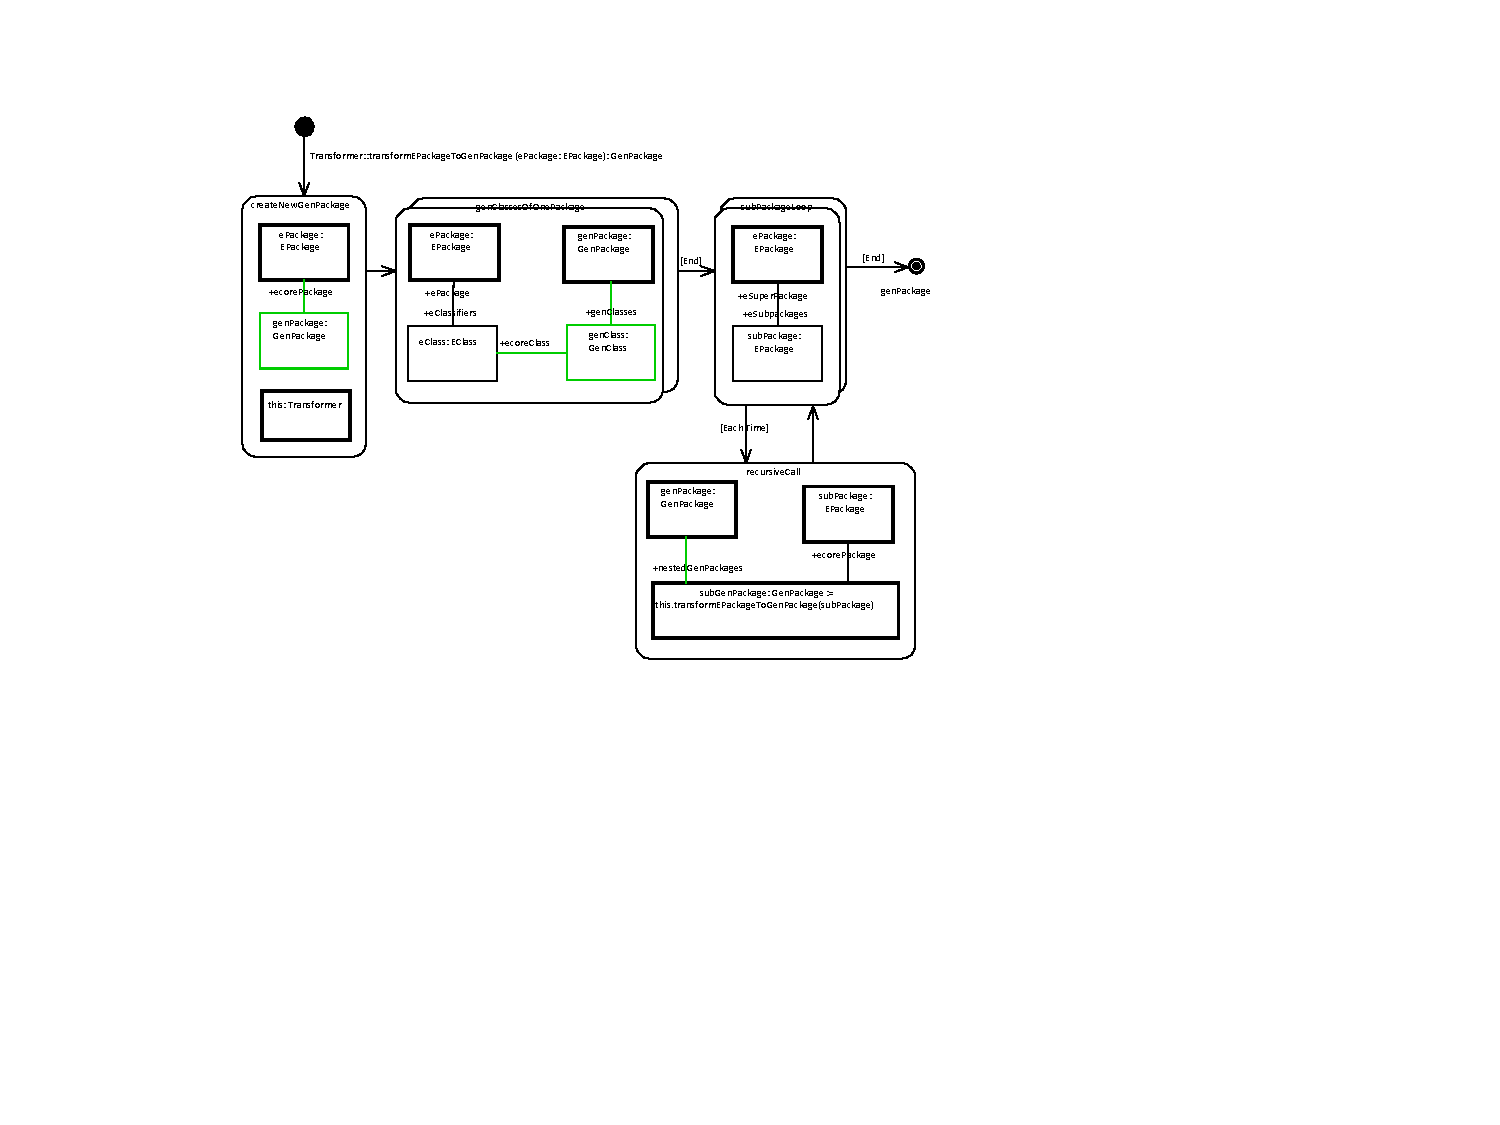
\includegraphics[width=1.1\textwidth]{SDMtransformEpackageToGenPackage.pdf}
\caption{Helper function to transform all \texttt{EPackages} to \texttt{GenPackages}}  
\label{fig_transf}
\end{center}
\end{figure} 

